\section{ PlanesAndroid }

\subsection { Navigation }

The Android App is built around the so-called Drawer Navigation. This kind of navigation is based on a so-called Hamburger button which in case of the Planes App is displayed in the top left corner of the screen. Tapping on the button displays a list possible destinations in the application. These depend on whether the app is played in the Single Player or Multiplayer Mode. 

In the case of the Single Player App we have:
\begin{itemize}
\item Game
\item Videos
\item Settings
\item Info
\end{itemize}

For the Multiplayer App more screens are available:

\begin{itemize}
	\item Game
	\item Connect to Game
	\item Game Statistics
	\item Login
	\item Logout
	\item Register
	\item Delete User
	\item Videos
	\item Settings
	\item Info
\end{itemize}

When a screen is selected, a Fragment of the Fragment Class corresponding to the screen is loaded into the main layout of the application. The XML layout of the application is shown in \ref{drawer_layout}.

To exemplify how a new screen is loaded onto the screen I show the following function ( \ref{start_norobot_fragment}).

\begin{lstlisting} [caption = {Switch Screen Example},label=start_norobot_fragment]
	fun startNoRobotFragment(regResp : RegistrationResponse) {
		
		mSelectedItem = R.id.nav_norobot  
		
		val newFragment = NoRobotFragment()
		val bundle = Bundle()
		bundle.putString("norobot/requestid", regResp.m_Id)
		bundle.putString("norobot/question", regResp.m_Question)
		val images =  arrayOf(regResp.m_ImageId_1, regResp.m_ImageId_2, regResp.m_ImageId_3, regResp.m_ImageId_4, regResp.m_ImageId_5,
		regResp.m_ImageId_6, regResp.m_ImageId_7, regResp.m_ImageId_8, regResp.m_ImageId_9)
		bundle.putSerializable("norobot/images", images)
		val selection = arrayOf(false, false, false, false, false, false, false, false, false)
		bundle.putSerializable("norobot/selection", selection)
		
		newFragment.arguments = bundle
		
		supportFragmentManager.beginTransaction()
		.replace(R.id.main_content, newFragment, ApplicationScreens.NoRobot.toString())
		.setTransition(FragmentTransaction.TRANSIT_FRAGMENT_FADE)
		.addToBackStack("FromRegister")
		.commit()
		
	}
	
\end{lstlisting}

This code shows the preparation for the start of the fragment called NoRobotFragment, which is the validation window to determine that the user is human. In the variable bundle the parameters that are to be given to the fragment are prepared. The actual switch of the screen is the call supportFragmentManager.beginTransaction(). Specifying R.id.main\_content defines where in the Drawer Layout should the new screen be displayed.  

\subsection { Android Concepts }

\subsubsection { Activity }

Activity is a central class in an Android app. In an activity the appearance of the app is defined through an XML layout. Also the behaviour of the app as response to variouse events in the app life cycle are defined in the activity.

For example the layout of the Planes Android app is as follows:

\begin{lstlisting} [caption = {App Drawer Layout},label=drawer_layout]

<?xml version="1.0" encoding="utf-8"?>
	<androidx.drawerlayout.widget.DrawerLayout
	xmlns:android="http://schemas.android.com/apk/res/android"
	xmlns:app="http://schemas.android.com/apk/res-auto"
	android:id="@+id/drawer_layout"
	android:layout_width="match_parent"
	android:layout_height="match_parent"
	android:fitsSystemWindows="true">
		<RelativeLayout
		android:layout_width="match_parent"
		android:layout_height="match_parent">
			<androidx.appcompat.widget.LinearLayoutCompat
				android:id="@+id/coordinator_id"
				android:layout_width="match_parent"
				android:layout_height="match_parent"
				android:orientation="vertical"
				android:background="@drawable/background">
				<com.google.android.material.appbar.AppBarLayout
				android:layout_width="match_parent"
				android:layout_height="wrap_content"
				android:theme="@style/ThemeOverlay.AppCompat.Dark.ActionBar">
				<androidx.appcompat.widget.Toolbar
				android:id="@+id/toolbar"
				android:layout_width="match_parent"
				android:layout_height="?attr/actionBarSize"
				app:theme="@style/MyToolbarTheme"
				app:layout_scrollFlags="enterAlways|scroll" />
				</com.google.android.material.appbar.AppBarLayout>
				<androidx.appcompat.widget.LinearLayoutCompat
				android:id="@+id/main_content"
				android:layout_width="match_parent"
				android:layout_height="match_parent"
				app:layout_behavior="@string/appbar_scrolling_view_behavior"/>
			</androidx.appcompat.widget.LinearLayoutCompat>
			<ProgressBar
			android:id="@+id/ProgressBarBottom"
			android:layout_width="350dp"
			android:layout_centerInParent="true"
			android:layout_height="350dp"
			android:foregroundTint="?planesProgressBarColor"
			android:progressTint="?planesProgressBarColor"
			android:indeterminateTint="?planesProgressBarColor"
			android:visibility="invisible" />
			<TextView
			android:id="@+id/LoaderLabelBottom"
			android:layout_width="wrap_content"
			android:layout_height="wrap_content"
			android:layout_margin="10dip"
			android:layout_alignParentBottom="true"
			android:textSize="20sp"
			android:textStyle="bold"
			style="@style/CustomTextViewStyle"
			android:text="@string/loader_text"
			android:visibility="invisible"/>
		</RelativeLayout>
	<com.google.android.material.navigation.NavigationView
	android:id="@+id/nav_view"
	android:layout_width="wrap_content"
	android:layout_height="wrap_content"
	android:layout_gravity="left"
	android:background="@drawable/background"
	app:menu="@menu/main_menu"
	app:theme="@style/NavigationDrawerStyle"
	app:headerLayout="@layout/nav_header"
	/>
	</androidx.drawerlayout.widget.DrawerLayout>
\end{lstlisting}
 
This xml defines the layout as a special type of layout: DrawerLayout. This includes the NavigationView which is the part of the layout which appears when clicking on the Hamburger button and allows the navigation to the different screens of the app. The content of the main activity screen is contained inside a RelativeLayout. In this layout are included a general use Progress Bar which is normally disabled but appears when different network calls are being made, the toolbar of the app and a placeholder for the different screens marked with the id main\_content.

\subsubsection { Activity Life Cycle }

\tikzstyle{startstop} = [rectangle, rounded corners, minimum width=3cm, 
minimum height=1cm, text centered, draw=black, fill=red!30]
\tikzstyle{process} = [rectangle, minimum width=3cm, minimum height=1cm, text centered, draw=black, fill=orange!30]
\tikzstyle{processb} = [rectangle, minimum width=3cm, minimum height=1cm, text centered, draw=black, fill=blue!30]
\tikzstyle{comment} = [rectangle, minimum width=3cm, minimum height=1cm, text centered,
text width=4cm, draw=white, fill=white]
\tikzstyle{arrow} = [thick,->,>=stealth]

\begin{figure}
	\caption{Activity Life Cycle diagram as it is presented on the Android developer pages}
	\label{fig:activity_life_cycle}
	\centering
		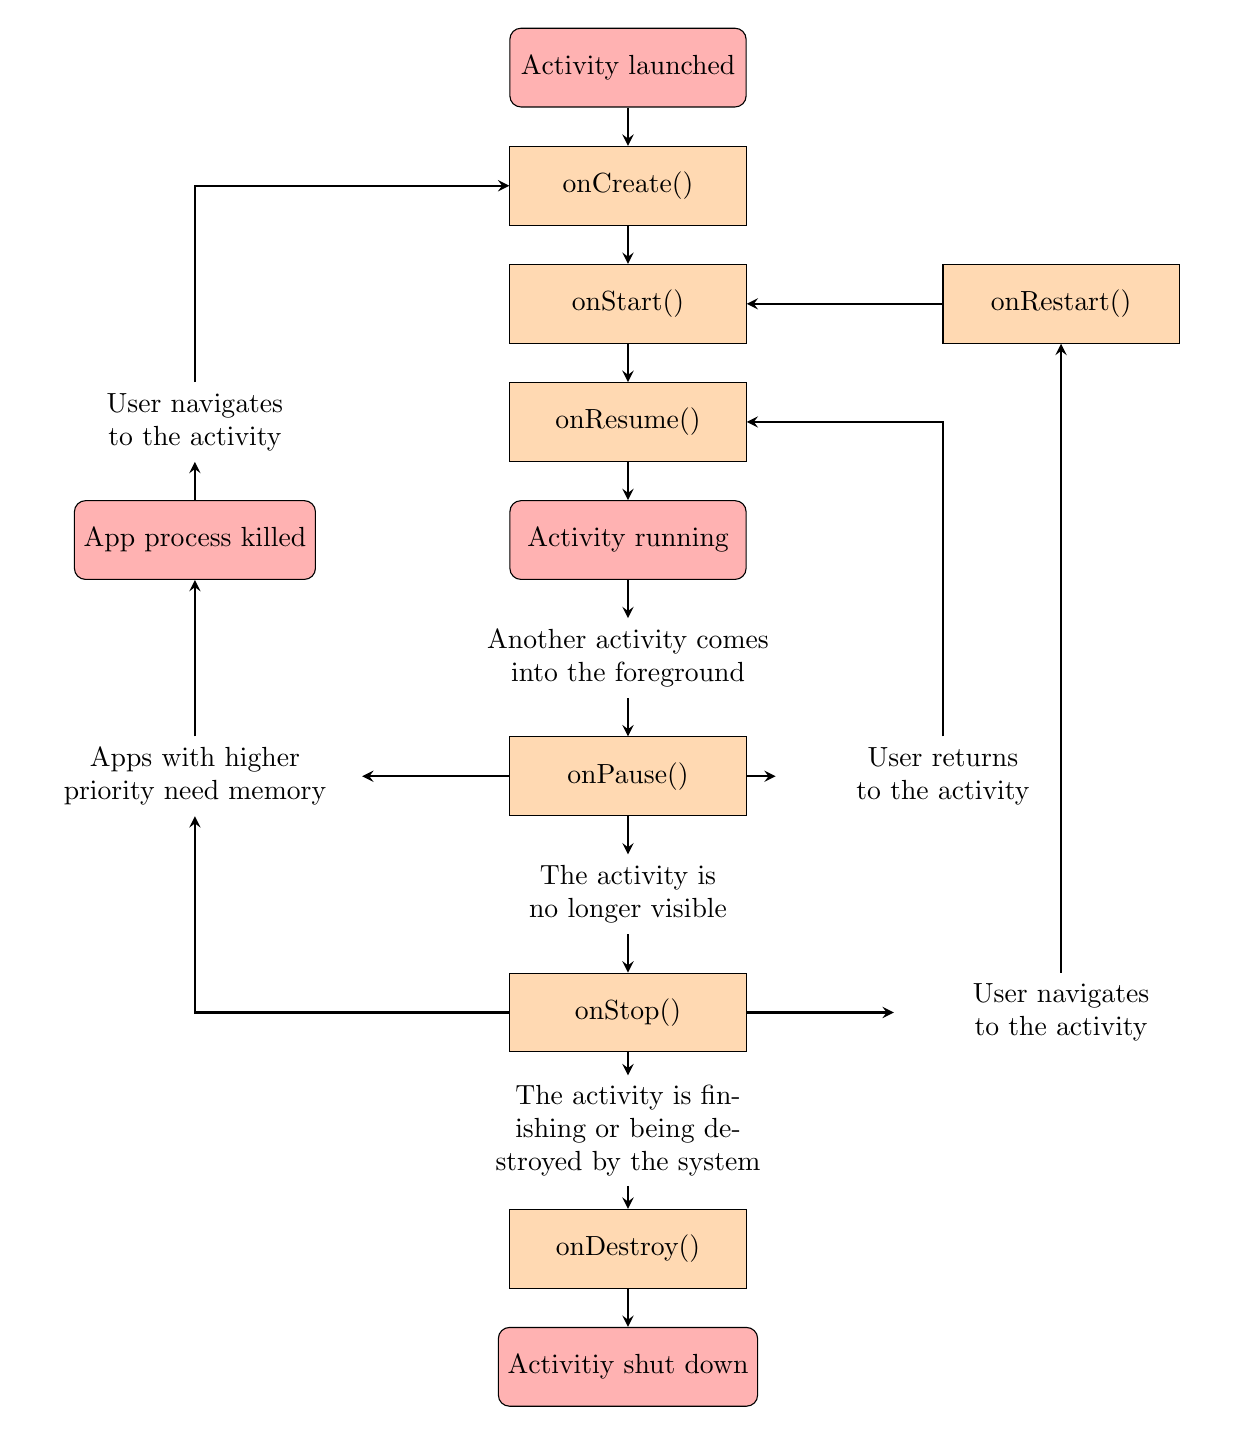
\begin{tikzpicture}[node distance=1.5cm]
			\node (start) [startstop] {Activity launched};
			\node (onCreate) [process, below of=start] {onCreate()};
			\node (onStart) [process, below of=onCreate] {onStart()};
			\node (onResume) [process, below of=onStart] {onResume()};
			\node (running) [startstop, below of=onResume] {Activity running};
			\node (commentOnPause) [comment, below of= running] {Another activity comes into the foreground};
			\node (onPause) [process, below of=commentOnPause] {onPause()};
			\node (commentOnStop) [comment, below of= onPause] {The activity is no longer visible};
			\node (onStop) [process, below of=commentOnStop] {onStop()};
			\node (commentOnDestroy) [comment, below of= onStop] {The activity is finishing or being destroyed by the system};
			\node (onDestroy) [process, below of=commentOnDestroy] {onDestroy()};
			\node (end) [startstop, below of=onDestroy] {Activitiy shut down};
			\node (onRestart) [process, right of=onStart, xshift=4cm] {onRestart()};
			\node (commentOnRestart) [comment, right of= onStop, xshift=4cm] {User navigates to the activity};
			\node (commentOnPauseRight) [comment, right of= onPause, xshift=2.5cm] {User returns to the activity};
			\node (commentOnPauseLeft) [comment, left of= onPause, xshift=-4cm] {Apps with higher priority need memory};
			\node (commentOnResumeLeft) [comment, left of= onResume, xshift=-4cm] {User navigates to the activity};
			\node (killed) [startstop, left of = running, xshift=-4cm] {App process killed};
			
			\draw [arrow] (start) -- (onCreate);
			\draw [arrow] (onCreate) -- (onStart);
			\draw [arrow] (onStart) -- (onResume);
			\draw [arrow] (onResume) -- (running);
			\draw [arrow] (running) -- (commentOnPause);
			\draw [arrow] (commentOnPause)  -- (onPause);
			\draw [arrow] (onPause) -- (commentOnStop);
			\draw [arrow] (commentOnStop) -- (onStop);
			\draw [arrow] (onStop) -- (commentOnDestroy);
			\draw [arrow] (commentOnDestroy) -- (onDestroy);
			\draw [arrow] (onDestroy) -- (end);
			\draw [arrow] (onRestart) -- (onStart);
			\draw [arrow] (onStop) -- (commentOnRestart);
			\draw [arrow] (commentOnRestart) -- (onRestart);
			\draw [arrow] (onPause) -- (commentOnPauseRight);
			\draw [arrow] (commentOnPauseRight) |- (onResume);
			\draw [arrow] (onPause) -> (commentOnPauseLeft);
			\draw [arrow] (onStop) -| (commentOnPauseLeft);
			\draw [arrow] (commentOnPauseLeft) -> (killed);
			\draw [arrow] (killed) -> (commentOnResumeLeft);
			\draw [arrow]  (commentOnResumeLeft) |- (onCreate);
			
		\end{tikzpicture}

\end{figure}

In figure \ref{fig:activity_life_cycle} one can see how various functions of the activity class are called depending in which state is the activity in following interaction with the user or with the Android operating system. The programmer has the possibilty to override these functions in order to customize the behaviour of the application.

In the following I will exemplify some of the methods as they are implemented in the Planes App. 

\begin{lstlisting} [caption = {onStop() life-cycle method},label=onStop_Android]
	override fun onStop() {
		m_SinglePlayerPreferencesService.writePreferences()
		m_MultiplayerPreferencesService.writePreferences()
		m_MainPreferencesService.writePreferences()
		m_VideoSettingsService.writePreferences()
		m_PlayersListService.stopPolling()
		m_ReceiveChatMessagesService.stopPolling()
		updateDatabaseFromNewMessagesFlags()
		super.onStop()
		Log.d("Planes", "onStop")
	}
\end{lstlisting}

In the onStop() method different screen configurations are saved in the so-called preferences of the app through calls of the method writePreferences(). The polling for the list of active players is stopped as well. The ROOM database is also updated with the information about the new messages.

\begin{lstlisting} [caption = {onResume() life-cycle method},label=onResume_Android]
	public override fun onResume() {
		super.onResume()
		if (m_MainPreferencesService.multiplayerVersion && m_MultiplayerRound.isUserLoggedIn()) {
			m_PlayersListService.startPolling()
			m_ReceiveChatMessagesService.startPolling()
			m_ReceiveChatMessagesService.setMainActivityUpdateFunction { updateNewMessagesFlags() }
		}
	}
\end{lstlisting}

In the onResume() method several configurations are made only for the the case when the user plays the multiplayer version and it is loogged in. These are:

\begin{itemize}
	\item Start polling for players' status
	\item Start polling for chat messages
	\item Configure the update of the main screen when receiving chat messages
	\item Update new messages flags on the top bar of the app
\end{itemize}


\subsubsection { Fragment }

Fragments represent a reusable portion of the UI. They are defined by their own layout files and have their own life cycle. They are hosted inside another fragment or an activity.

\subsubsection { Fragment Life Cycle }

\begin{figure}
	\caption{Fragment Life Cycle diagram as it is presented on the Android developer pages}
	\label{fig:fragment_life_cycle}
	\centering
	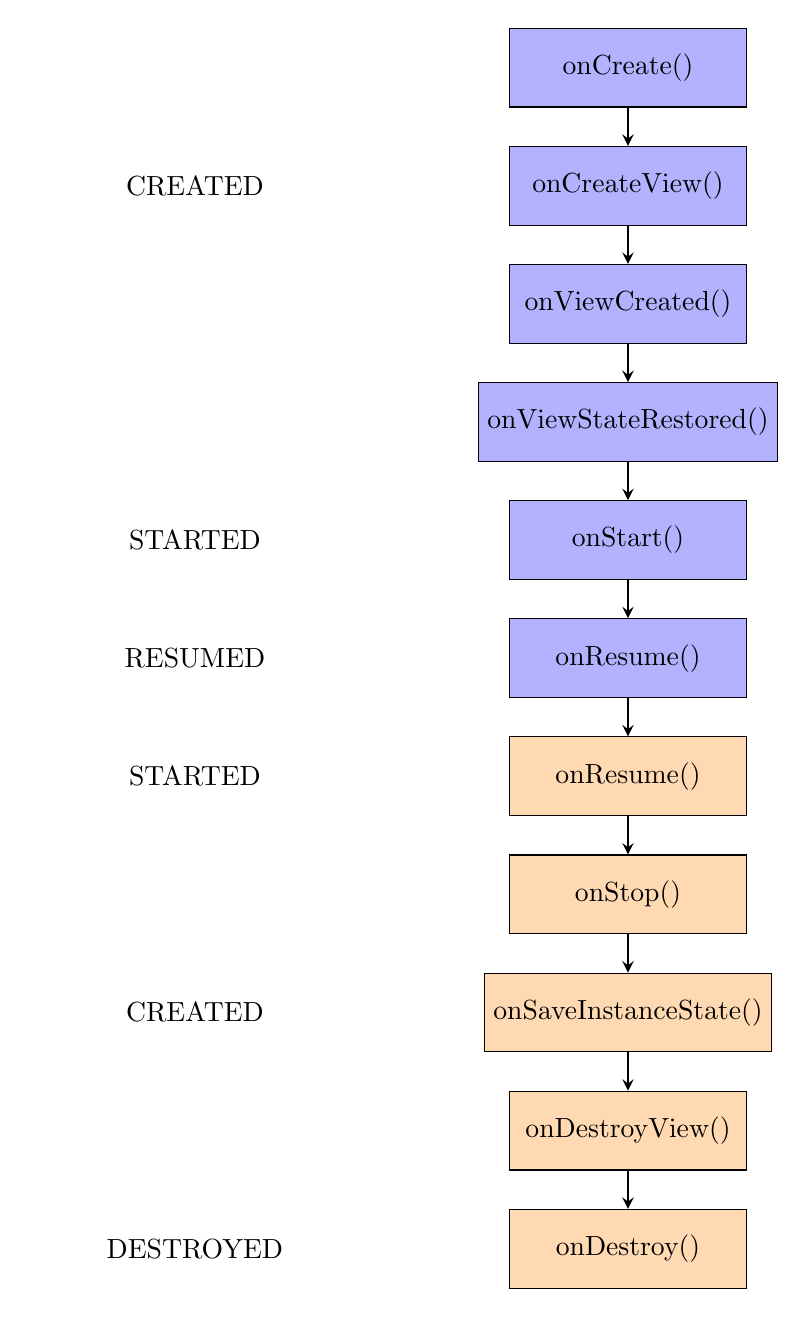
\begin{tikzpicture}[node distance=1.5cm]
		\node (onCreate) [processb] {onCreate()};
		\node (onCreateView) [processb, below of=onCreate] {onCreateView()};
		\node (onViewCreated) [processb, below of=onCreateView] {onViewCreated()};
		\node (onViewStateRestored) [processb, below of=onViewCreated] {onViewStateRestored()};
		\node (onStart) [processb, below of=onViewStateRestored] {onStart()};
		\node (onResume) [processb, below of= onStart] { onResume() };
		\node (onPause) [process, below of=onResume] {onResume()};
		\node (onStop) [process, below of= onPause] {onStop()};
		\node (onSaveInstanceState) [process, below of=onStop] {onSaveInstanceState()};
		\node (onDestroyView) [process, below of= onSaveInstanceState] {onDestroyView()};
		\node (onDestroy) [process, below of=onDestroyView] {onDestroy()};
		
		\node (ccreated) [comment, left of = onCreateView, xshift = -4cm] {CREATED};
		\node (cstarted) [comment, left of = onStart, xshift = -4cm] {STARTED};
		\node (cresumed) [comment, left of = onResume, xshift = -4cm] {RESUMED};
		\node (cstarted1) [comment, left of = onPause, xshift = -4cm] {STARTED};
		\node (ccreated1) [comment, left of = onSaveInstanceState, xshift = -4cm] {CREATED};
		\node (cdestroyed) [comment, left of = onDestroy, xshift = -4cm] {DESTROYED};
		
		\draw [arrow] (onCreate) -- (onCreateView);
		\draw [arrow] (onCreateView) -- (onViewCreated);
		\draw [arrow] (onViewCreated) -- (onViewStateRestored);
		\draw [arrow] (onViewStateRestored) -- (onStart);
		\draw [arrow] (onStart) -- (onResume);
		\draw [arrow] (onResume) -- (onPause);
		\draw [arrow] (onPause) -- (onStop);
		\draw [arrow] (onStop) -- (onSaveInstanceState);
		\draw [arrow] (onSaveInstanceState) -- (onDestroyView);
		\draw [arrow] (onDestroyView) -- (onDestroy);
	
	\end{tikzpicture}
	
\end{figure}


\section{PlanesCompose}

Following new developments of Android development libraries I am porting the project to a new technology: JetPack Compose. 

\subsection{Navigation}

The basis of the application is the navigation. Here I wish to keep the drawer navigation. 
The navigation drawer and main screen content are defined as follows (\ref{drawer_compose})

\begin{lstlisting}  [caption = {Drawer Navigation in Jetpack Compose},label=drawer_compose]
	ModalNavigationDrawer(
	drawerState = drawerState,
	drawerContent = {
		ModalDrawerSheet {
			DrawerContent(navController = navController,
			drawerScope = scope,
			drawerState = drawerState)
		}
	},
	gesturesEnabled = true
	) {
		Scaffold(
		topBar = {
			TopBar(
			modifier = Modifier.padding(30.dp)
			.height(100.dp).fillMaxWidth(),
			onOpenDrawer = {
				scope.launch {
					drawerState.apply {
						if (isClosed)
						open()
						else
						close()
					}
				}
			},
			currentScreenName = currentScreenState.value
			)
		}
		) { padding ->
			ScreenContent(modifier = Modifier.padding(padding),
			currentScreenState = currentScreenState,
			navController = navController)
		}
	}
\end{lstlisting}

The design of the drawer is definedUnder the drawer\_content variable. The layout of the application screen is defined under the ending lambda of the ModalNavigationDrawer composable . 

In listing \ref{drawer_layout__compose} the structure of the drawer is shown. Probably this is not the final code for the drawer but the principle will stay the same. So the drawer is a Column layout in which screen names are stacked one under another. The screen names are grouped in sections and a HorizontalDivider is shown between sections .

\begin{lstlisting} [caption = {Drawer View},label=drawer_layout__compose]
	@Composable
	fun DrawerContent(modifier: Modifier = Modifier,
	navController: NavController,
	drawerScope: CoroutineScope,
	drawerState: DrawerState,
	) {
		
		Column(
		modifier = Modifier.padding(horizontal = 16.dp)
		.verticalScroll(rememberScrollState())
		) {
			Text(
			text = "Planes",
			modifier = Modifier.padding(16.dp),
			style = MaterialTheme.typography.titleLarge
			)
			
			HorizontalDivider()
			
			DrawerMenuItemGeneric("Login", {
				drawerScope.launch {
					drawerState.close()
				}
				navController.navigate(route = PlanesScreens.Login.name)
			})
			
			DrawerMenuItemGeneric("Logout", {
				drawerScope.launch {
					drawerState.close()
				}
				navController.navigate(route = PlanesScreens.Logout.name)
			})
			
			DrawerMenuItemGeneric("Register", {
				drawerScope.launch {
					drawerState.close()
				}
				navController.navigate(route = PlanesScreens.Register.name)
			})
			
			DrawerMenuItemGeneric("Chat", {
				drawerScope.launch {
					drawerState.close()
				}
				navController.navigate(route = PlanesScreens.Chat.name)
			})
			
			Text(
			text = "Single Player Game",
			modifier = Modifier.padding(16.dp),
			style = MaterialTheme.typography.titleMedium
			)
			DrawerMenuItemGeneric("Game", {
				drawerScope.launch {
					drawerState.close()
				}
				navController.navigate(route = PlanesScreens.SinglePlayerGame.name)
			})
			
			DrawerMenuItemGeneric("Preferences", {
				drawerScope.launch {
					drawerState.close()
				}
				navController.navigate(route = PlanesScreens.SinglePlayerPreferences.name)
			})
			
			DrawerMenuItemGeneric("Game Statistics", {
				drawerScope.launch {
					drawerState.close()
				}
				navController.navigate(route = PlanesScreens.SinglePlayerGameStatistics.name)
			})
			
			
			Text(
			text = "Multiplayer Game",
			modifier = Modifier.padding(16.dp),
			style = MaterialTheme.typography.titleMedium
			)
			DrawerMenuItemGeneric("Game", {
				drawerScope.launch {
					drawerState.close()
				}
				navController.navigate(route = PlanesScreens.MultiplayerGame.name)
			})
			
			DrawerMenuItemGeneric("Preferences", {
				drawerScope.launch {
					drawerState.close()
				}
				navController.navigate(route = PlanesScreens.MultiplayerPreferences.name)
			})
			
			DrawerMenuItemGeneric("Game Statistics", {
				drawerScope.launch {
					drawerState.close()
				}
				navController.navigate(route = PlanesScreens.MultiplayerGameStatistics.name)
			})
			
			Text(
			text = "Info",
			modifier = Modifier.padding(16.dp),
			style = MaterialTheme.typography.titleMedium
			)
			
			DrawerMenuItemGeneric("About", {
				drawerScope.launch {
					drawerState.close()
				}
				navController.navigate(route = PlanesScreens.Info.name)
			})
			
			DrawerMenuItemGeneric("Tutorials", {
				drawerScope.launch {
					drawerState.close()
				}
				navController.navigate(route = PlanesScreens.Tutorials.name)
			})
			
			DrawerMenuItemGeneric("Delete User", {
				drawerScope.launch {
					drawerState.close()
				}
				navController.navigate(route = PlanesScreens.DeleteUser.name)
			})
		}
	}
\end{lstlisting}

Each screen name is represented by an element of the composable DrawerMenuItemGeneric which receive parameters the screen name and a lambda function that it is to be called when the screen name is clicked. The call navController.navigate() makes the screen transition. It corresponds to the supportFragmentManager.beginTransaction() from \ref{start_norobot_fragment}.

\subsection{Main Screen}

The structure of the application screen is also defined in listing \ref{drawer_compose} which is the definition of the drawer navigation. This is defined with a Scaffold composable composed of a top bar together with the content of the screen.

\begin{lstlisting} [caption = {Main Screen Layout},label=main_screen]
	Scaffold(
	topBar = {
		TopBar(
		modifier = Modifier.padding(30.dp)
		.height(100.dp).fillMaxWidth(),
		onOpenDrawer = {
			scope.launch {
				drawerState.apply {
					if (isClosed)
					open()
					else
					close()
				}
			}
		},
		currentScreenName = currentScreenState.value
		)
	}
	) { padding ->
		ScreenContent(modifier = Modifier.padding(padding),
		currentScreenState = currentScreenState,
		navController = navController)
	}
\end{lstlisting} 

TopBar is defined as follows:

\begin{lstlisting}  [caption = {Top Bar},label=top_bar]
	TopBar(modifier: Modifier = Modifier,
	onOpenDrawer: () -> Unit = {},
	currentScreenName: String
	) {
		TopAppBar(
		colors = TopAppBarDefaults.topAppBarColors(
		containerColor = MaterialTheme.colorScheme.surfaceVariant
		),
		navigationIcon = {
			Icon(
			imageVector = Icons.Default.Menu,
			contentDescription = "Navigation Icon",
			modifier = Modifier.clickable {
				onOpenDrawer()
			}. padding(start = 16.dp, end = 8.dp)
			.size(28.dp))
		},
		title = {
			Text(text = currentScreenName)
		},
		actions = {
			Icon(
			imageVector = Icons.Default.AccountBox,
			contentDescription = "Navigation Icon",
			modifier = Modifier.padding(start = 16.dp, end = 8.dp).size(28.dp)
			)
			Icon(
			imageVector = Icons.Default.Notifications,
			contentDescription = "Navigation Icon",
			modifier = Modifier.padding(start = 16.dp, end = 8.dp)
			.size(28.dp))
		}
		)
	}
	
\end{lstlisting}

This uses the predefined composable TopAppBar which receives as parameters a navigation icon (the Hamburger button), the title displayed as well as actions which can be added to this bar to be called from everywhere in the app. The variable currentScreenName is defined such that when a new screen is shown the title of the screen is displayed in the top bar.

The ScreenContent composable defines the changing content of the main screen as follows:

\begin{lstlisting}
	@Composable
	fun ScreenContent(modifier: Modifier, currentScreenState: MutableState<String>,
	navController: NavHostController
	) {
		PlanesNavigation(modifier = modifier,
		currentScreenState, navController,
		context = LocalContext.current)
	}
\end{lstlisting}

PlanesNavigation is a composable that associates to the application screen names composable functions representing the respective screens.

\begin{lstlisting}
	@Composable
	fun PlanesNavigation(modifier: Modifier, currentScreenState: MutableState<String>,
	navController: NavHostController, context: Context) {
		
		NavHost(
		navController = navController,
		startDestination = PlanesScreens.Info.name) {
			composable(PlanesScreens.SinglePlayerGame.name) {
				SinglePlayerGameScreen(modifier = modifier, currentScreenState, navController = navController)
			}
			composable(PlanesScreens.SinglePlayerGameStatistics.name) {
				SinglePlayerGameStatisticsScreen(modifier = modifier, currentScreenState, navController = navController)
			}
			composable(PlanesScreens.SinglePlayerPreferences.name) {
				SinglePlayerPreferencesScreen(modifier = modifier, currentScreenState, navController = navController)
			}
			composable(PlanesScreens.MultiplayerGame.name) {
				MultiplayerGameScreen(modifier = modifier, currentScreenState, navController = navController)
			}
			composable(PlanesScreens.MultiplayerGameStatistics.name) {
				MultiplayerGameStatisticsScreen(modifier = modifier, currentScreenState, navController = navController)
			}
			composable(PlanesScreens.MultiplayerPreferences.name) {
				MultiplayerPreferencesScreen(modifier = modifier, currentScreenState, navController = navController)
			}
			composable(PlanesScreens.Info.name) {
				AboutScreen(modifier = modifier, currentScreenState, navController = navController,
				aboutEntryList = AboutEntryRepository.create("0.1", context = context))
			}
			composable(PlanesScreens.Tutorials.name) {
				VideoScreen(modifier = modifier, currentScreenState, navController = navController)
			}
			composable(PlanesScreens.Login.name) {
				LoginScreen(modifier = modifier, currentScreenState, navController = navController)
			}
			composable(PlanesScreens.Logout.name) {
				LogoutScreen(modifier = modifier, currentScreenState, navController = navController)
			}
			composable(PlanesScreens.Register.name) {
				RegisterScreen(modifier = modifier, currentScreenState, navController = navController)
			}
			composable(PlanesScreens.DeleteUser.name) {
				DeleteUserScreen(modifier = modifier, currentScreenState, navController = navController)
			}
			composable(PlanesScreens.Chat.name) {
				ChatScreen(modifier = modifier, currentScreenState, navController = navController)
			}
		}
\end{lstlisting}